% Options for packages loaded elsewhere
\PassOptionsToPackage{unicode}{hyperref}
\PassOptionsToPackage{hyphens}{url}
%
\documentclass[
]{book}
\usepackage{amsmath,amssymb}
\usepackage{lmodern}
\usepackage{iftex}
\ifPDFTeX
  \usepackage[T1]{fontenc}
  \usepackage[utf8]{inputenc}
  \usepackage{textcomp} % provide euro and other symbols
\else % if luatex or xetex
  \usepackage{unicode-math}
  \defaultfontfeatures{Scale=MatchLowercase}
  \defaultfontfeatures[\rmfamily]{Ligatures=TeX,Scale=1}
\fi
% Use upquote if available, for straight quotes in verbatim environments
\IfFileExists{upquote.sty}{\usepackage{upquote}}{}
\IfFileExists{microtype.sty}{% use microtype if available
  \usepackage[]{microtype}
  \UseMicrotypeSet[protrusion]{basicmath} % disable protrusion for tt fonts
}{}
\makeatletter
\@ifundefined{KOMAClassName}{% if non-KOMA class
  \IfFileExists{parskip.sty}{%
    \usepackage{parskip}
  }{% else
    \setlength{\parindent}{0pt}
    \setlength{\parskip}{6pt plus 2pt minus 1pt}}
}{% if KOMA class
  \KOMAoptions{parskip=half}}
\makeatother
\usepackage{xcolor}
\IfFileExists{xurl.sty}{\usepackage{xurl}}{} % add URL line breaks if available
\IfFileExists{bookmark.sty}{\usepackage{bookmark}}{\usepackage{hyperref}}
\hypersetup{
  pdftitle={MBAn Career Handbook},
  pdfauthor={Keep Rolling},
  hidelinks,
  pdfcreator={LaTeX via pandoc}}
\urlstyle{same} % disable monospaced font for URLs
\usepackage{color}
\usepackage{fancyvrb}
\newcommand{\VerbBar}{|}
\newcommand{\VERB}{\Verb[commandchars=\\\{\}]}
\DefineVerbatimEnvironment{Highlighting}{Verbatim}{commandchars=\\\{\}}
% Add ',fontsize=\small' for more characters per line
\usepackage{framed}
\definecolor{shadecolor}{RGB}{248,248,248}
\newenvironment{Shaded}{\begin{snugshade}}{\end{snugshade}}
\newcommand{\AlertTok}[1]{\textcolor[rgb]{0.94,0.16,0.16}{#1}}
\newcommand{\AnnotationTok}[1]{\textcolor[rgb]{0.56,0.35,0.01}{\textbf{\textit{#1}}}}
\newcommand{\AttributeTok}[1]{\textcolor[rgb]{0.77,0.63,0.00}{#1}}
\newcommand{\BaseNTok}[1]{\textcolor[rgb]{0.00,0.00,0.81}{#1}}
\newcommand{\BuiltInTok}[1]{#1}
\newcommand{\CharTok}[1]{\textcolor[rgb]{0.31,0.60,0.02}{#1}}
\newcommand{\CommentTok}[1]{\textcolor[rgb]{0.56,0.35,0.01}{\textit{#1}}}
\newcommand{\CommentVarTok}[1]{\textcolor[rgb]{0.56,0.35,0.01}{\textbf{\textit{#1}}}}
\newcommand{\ConstantTok}[1]{\textcolor[rgb]{0.00,0.00,0.00}{#1}}
\newcommand{\ControlFlowTok}[1]{\textcolor[rgb]{0.13,0.29,0.53}{\textbf{#1}}}
\newcommand{\DataTypeTok}[1]{\textcolor[rgb]{0.13,0.29,0.53}{#1}}
\newcommand{\DecValTok}[1]{\textcolor[rgb]{0.00,0.00,0.81}{#1}}
\newcommand{\DocumentationTok}[1]{\textcolor[rgb]{0.56,0.35,0.01}{\textbf{\textit{#1}}}}
\newcommand{\ErrorTok}[1]{\textcolor[rgb]{0.64,0.00,0.00}{\textbf{#1}}}
\newcommand{\ExtensionTok}[1]{#1}
\newcommand{\FloatTok}[1]{\textcolor[rgb]{0.00,0.00,0.81}{#1}}
\newcommand{\FunctionTok}[1]{\textcolor[rgb]{0.00,0.00,0.00}{#1}}
\newcommand{\ImportTok}[1]{#1}
\newcommand{\InformationTok}[1]{\textcolor[rgb]{0.56,0.35,0.01}{\textbf{\textit{#1}}}}
\newcommand{\KeywordTok}[1]{\textcolor[rgb]{0.13,0.29,0.53}{\textbf{#1}}}
\newcommand{\NormalTok}[1]{#1}
\newcommand{\OperatorTok}[1]{\textcolor[rgb]{0.81,0.36,0.00}{\textbf{#1}}}
\newcommand{\OtherTok}[1]{\textcolor[rgb]{0.56,0.35,0.01}{#1}}
\newcommand{\PreprocessorTok}[1]{\textcolor[rgb]{0.56,0.35,0.01}{\textit{#1}}}
\newcommand{\RegionMarkerTok}[1]{#1}
\newcommand{\SpecialCharTok}[1]{\textcolor[rgb]{0.00,0.00,0.00}{#1}}
\newcommand{\SpecialStringTok}[1]{\textcolor[rgb]{0.31,0.60,0.02}{#1}}
\newcommand{\StringTok}[1]{\textcolor[rgb]{0.31,0.60,0.02}{#1}}
\newcommand{\VariableTok}[1]{\textcolor[rgb]{0.00,0.00,0.00}{#1}}
\newcommand{\VerbatimStringTok}[1]{\textcolor[rgb]{0.31,0.60,0.02}{#1}}
\newcommand{\WarningTok}[1]{\textcolor[rgb]{0.56,0.35,0.01}{\textbf{\textit{#1}}}}
\usepackage{longtable,booktabs,array}
\usepackage{calc} % for calculating minipage widths
% Correct order of tables after \paragraph or \subparagraph
\usepackage{etoolbox}
\makeatletter
\patchcmd\longtable{\par}{\if@noskipsec\mbox{}\fi\par}{}{}
\makeatother
% Allow footnotes in longtable head/foot
\IfFileExists{footnotehyper.sty}{\usepackage{footnotehyper}}{\usepackage{footnote}}
\makesavenoteenv{longtable}
\usepackage{graphicx}
\makeatletter
\def\maxwidth{\ifdim\Gin@nat@width>\linewidth\linewidth\else\Gin@nat@width\fi}
\def\maxheight{\ifdim\Gin@nat@height>\textheight\textheight\else\Gin@nat@height\fi}
\makeatother
% Scale images if necessary, so that they will not overflow the page
% margins by default, and it is still possible to overwrite the defaults
% using explicit options in \includegraphics[width, height, ...]{}
\setkeys{Gin}{width=\maxwidth,height=\maxheight,keepaspectratio}
% Set default figure placement to htbp
\makeatletter
\def\fps@figure{htbp}
\makeatother
\setlength{\emergencystretch}{3em} % prevent overfull lines
\providecommand{\tightlist}{%
  \setlength{\itemsep}{0pt}\setlength{\parskip}{0pt}}
\setcounter{secnumdepth}{5}
\usepackage{booktabs}
\ifLuaTeX
  \usepackage{selnolig}  % disable illegal ligatures
\fi
\usepackage[]{natbib}
\bibliographystyle{apalike}

\title{MBAn Career Handbook}
\author{Keep Rolling}
\date{2022-07-26}

\begin{document}
\maketitle

{
\setcounter{tocdepth}{1}
\tableofcontents
}
\hypertarget{introduction}{%
\chapter{Introduction}\label{introduction}}

This is a \emph{sample} book written in \textbf{Markdown}. You can use anything that Pandoc's Markdown supports; for example, a math equation \(a^2 + b^2 = c^2\).

\hypertarget{usage}{%
\section{Usage}\label{usage}}

Each \textbf{bookdown} chapter is an .Rmd file, and each .Rmd file can contain one (and only one) chapter. A chapter \emph{must} start with a first-level heading: \texttt{\#\ A\ good\ chapter}, and can contain one (and only one) first-level heading.

Use second-level and higher headings within chapters like: \texttt{\#\#\ A\ short\ section} or \texttt{\#\#\#\ An\ even\ shorter\ section}.

The \texttt{index.Rmd} file is required, and is also your first book chapter. It will be the homepage when you render the book.

\hypertarget{render-book}{%
\section{Render book}\label{render-book}}

You can render the HTML version of this example book without changing anything:

\begin{enumerate}
\def\labelenumi{\arabic{enumi}.}
\item
  Find the \textbf{Build} pane in the RStudio IDE, and
\item
  Click on \textbf{Build Book}, then select your output format, or select ``All formats'' if you'd like to use multiple formats from the same book source files.
\end{enumerate}

Or build the book from the R console:

\begin{Shaded}
\begin{Highlighting}[]
\NormalTok{bookdown}\SpecialCharTok{::}\FunctionTok{render\_book}\NormalTok{()}
\end{Highlighting}
\end{Shaded}

To render this example to PDF as a \texttt{bookdown::pdf\_book}, you'll need to install XeLaTeX. You are recommended to install TinyTeX (which includes XeLaTeX): \url{https://yihui.org/tinytex/}.

\hypertarget{preview-book}{%
\section{Preview book}\label{preview-book}}

As you work, you may start a local server to live preview this HTML book. This preview will update as you edit the book when you save individual .Rmd files. You can start the server in a work session by using the RStudio add-in ``Preview book'', or from the R console:

\begin{Shaded}
\begin{Highlighting}[]
\NormalTok{bookdown}\SpecialCharTok{::}\FunctionTok{serve\_book}\NormalTok{()}
\end{Highlighting}
\end{Shaded}

\hypertarget{about-us}{%
\chapter{About Us}\label{about-us}}

We are Team Keep Rolling, a group of MBAn students in the first-ever year of this new program! We chose this name to describe us because we went into this semester with the plan to never give up, continue to be creative and bring our ideas together for success!

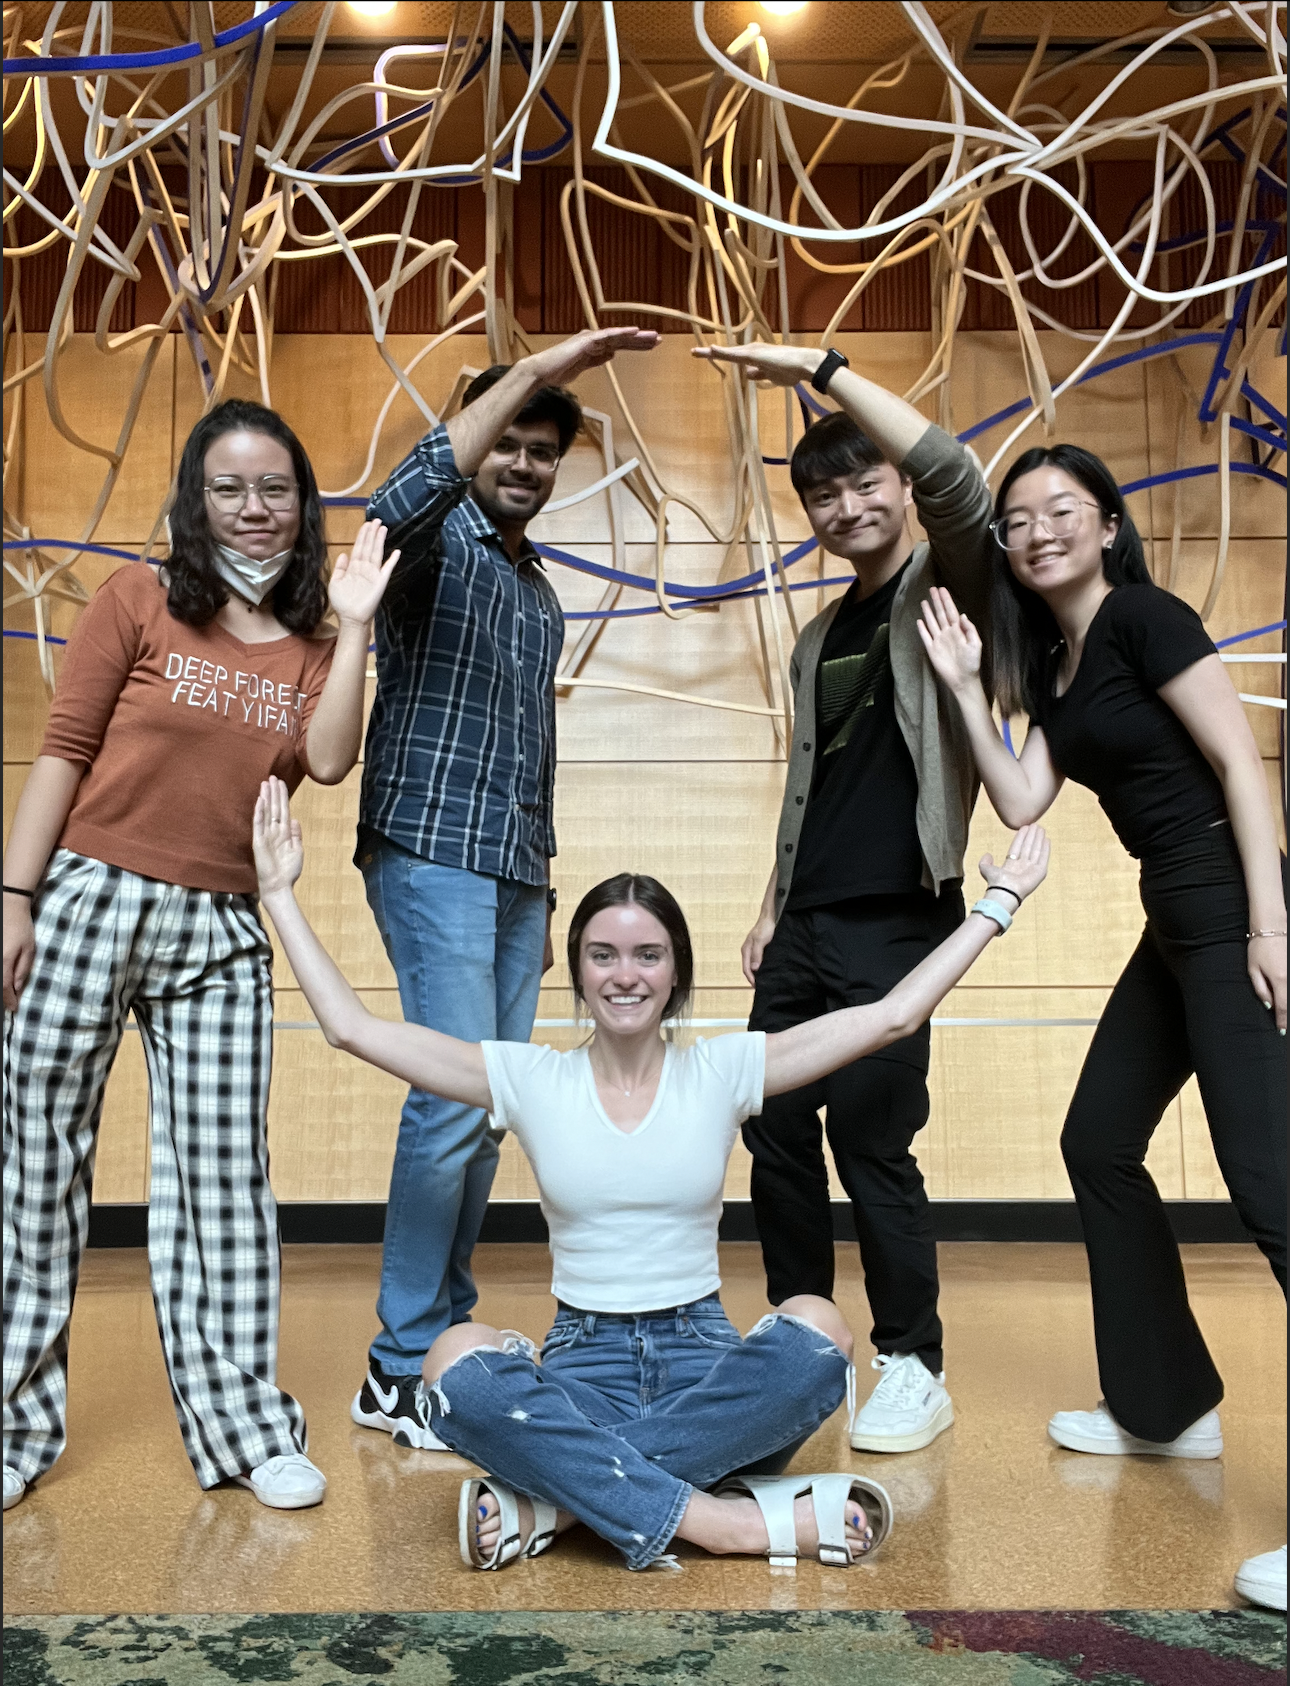
\includegraphics[width=0.5\textwidth,height=\textheight]{Images/group_pic.png}

As individuals, we bring lots of different skills and perspectives to this collective team and are motivated to learn more about career paths for this new program to serve future students. You can learn more about each of us in the sections to follow.

\hypertarget{amey-bhile}{%
\section{Amey Bhile}\label{amey-bhile}}

\includegraphics[width=0.5\textwidth,height=\textheight]{Images/Amey.jpeg}

\begin{quote}
Hey There, MBAn folk !! I'm Amey\\
I was born and brought up in India, where I also completed my Bachelor of Engineering in Computer Science, after which I worked as a technology consultant for three years. During my time at Deloitte, I realized my interests lie at the interface of technology and business; And I needed to expand my skills and knowledge in these domains, which is when I decided to join Ross Business School. ~
I wish to leverage data and apply ML/analytical frameworks to derive actionable insights and create value. I enjoy operating far outside my comfort zone and believe in the power of incremental improvements.\\
Feel free to reach out; I am always happy to help :)
\end{quote}

\begin{quote}
``Data is just summaries of thousands of stories - tell a few of them to the world, and you are a data analyst.''
\end{quote}

\hypertarget{eunguy-lee}{%
\section{Eunguy Lee}\label{eunguy-lee}}

\includegraphics[width=0.5\textwidth,height=\textheight]{1651691637018.jpg}

\begin{quote}
Hello everyone! This is Eunguy.\\
I was born in 1996 and grew up in South Korea. I went to Michigan State University and studied Supply Chain Management. After my junior year in college, I went back to South Korea to serve military as an operations sergeant for about two years. After the military experience, I finished my bechelor degree with online courses from MSU because of the pandemic. Meanwhile, I felt the need of capability handling data so I applied for graduate school with Business Analytics major.
\end{quote}

\begin{quote}
At this point at Ross, I am so exciting to build my network and equip myself with useful tools, such as Python, R, and SQL. As a business person, I am not used to these computer skills. However, someone said ``the pain that doesn't kill you will make you stronger.'' I believe putting my time and effort for the next 10 months will develop my ability as a business analyst. I hope this career handbook brings some insights for you.
\end{quote}

\hypertarget{snow-shen}{%
\section{Snow Shen}\label{snow-shen}}

\includegraphics[width=0.5\textwidth,height=\textheight]{Images/Snow.png}

\begin{quote}
Hi, I'm Snow! I come from a southern city in China called Hangzhou. It's warm there and seldomly snows. Every winter, I waited for snow and hoped the world can be covered in white when I wake up. That's why my parents gave me the English name Snow. I went to US in 2019 for my undergrad study. Boston was my destination due to the attractiveness of snow. I spent three years at Boston and then moved to Ann Arbor for graduate study. People hate the long winter here, but I am looking forward to it!
\end{quote}

\hypertarget{mary-silvio}{%
\section{Mary Silvio}\label{mary-silvio}}

\includegraphics[width=0.5\textwidth,height=\textheight]{Images/Mary.JPEG}

\begin{quote}
I am a self-proclaimed true Midwestern girl that grew up in Livonia, Michigan (perfectly halfway between Ann Arbor and Detroit). I graduated from the University of Michigan College of Engineering in Spring 2022 with a B.S.E. in Chemical Engineering and am a current Master's of Business Analytics student at the Stephen M. Ross School of Business. If there is one thing I took away from my undergraduate years, it is that the world will never run out of ways to improve, and thus never run out of problems to solve. Pushing the bounds of knowledge is what allows us to improve the systems around us, and that is why I value the potential of harnessing data - bringing me to the MBAn program to build my analytic skills to give data power.
\end{quote}

\begin{quote}
I have experience working in Chemical Manufacturing, Engineering Research, and Higher Education. Outside of school, I love going to SoulCycle, going on walks with friends, watching Detroit sports, trying new coffee shops, and cooking! It is my dream to be an analyst by day, and cycling instructor by night.
\end{quote}

\hypertarget{ziye-wang}{%
\section{Ziye Wang}\label{ziye-wang}}

\includegraphics[width=0.5\textwidth,height=\textheight]{Photo3.jpg}

\begin{quote}
My name is Ziye Wang, from Beijing, China. I graduated from the Central University of Finance and Economics in China, majoring in Financial Engineering.After graduation, I joined Capgemini Invent as an associate consultant, focused on auto and digital transformation.
\end{quote}

\begin{quote}
Something interesting about me I'd like to share with you:
I like drinking more than I like soup
I have 3 cute little nephews and my favorite thing to do on weekends is to play with my little nephew
I'm a Cancer girl but I'm more of a Leo
I lost weight for 5 years but never succeeded
\end{quote}

\begin{quote}
I'm very happy to be part of the Ross community. Hopefully our work will be helpful to everyone.
\end{quote}

\hypertarget{why-choose-the-mban-program-at-ross}{%
\chapter{Why Choose the MBAn Program at Ross?}\label{why-choose-the-mban-program-at-ross}}

We can also add our group photo for this page

\hypertarget{program-value}{%
\section{Program Value}\label{program-value}}

\hypertarget{coursework}{%
\section{Coursework}\label{coursework}}

\hypertarget{career-resources}{%
\section{Career Resources}\label{career-resources}}

\hypertarget{career-development-office}{%
\subsection{Career Development Office}\label{career-development-office}}

\hypertarget{other-ross-resources}{%
\subsection{Other Ross Resources}\label{other-ross-resources}}

\hypertarget{long-term-gains}{%
\section{Long-Term Gains}\label{long-term-gains}}

\hypertarget{career-choices}{%
\chapter{Career Choices}\label{career-choices}}

\hypertarget{expected-career-outcomes}{%
\section{Expected Career Outcomes}\label{expected-career-outcomes}}

\begin{quote}
This is the list of the major career choices after a Business analytics program.
\end{quote}

\begin{itemize}
\tightlist
\item
  Business Analyst Consultant
\item
  Product Management
\item
  Business Analyst/Data Scientist
\item
\end{itemize}

\hypertarget{business-analyst-consultant}{%
\subsection{Business Analyst Consultant}\label{business-analyst-consultant}}

\hypertarget{product-management}{%
\subsection{Product Management}\label{product-management}}

\hypertarget{business-analyst}{%
\subsection{Business Analyst}\label{business-analyst}}

\hypertarget{data-scientist}{%
\subsection{Data scientist}\label{data-scientist}}

\begin{itemize}
\item
  Who -
\item
  What -
\item
  How -
\item
  Companies -
\item
  Salary Range -
\item ~
  \hypertarget{data-engineer}{%
  \subsection{Data Engineer}\label{data-engineer}}
\end{itemize}

\includegraphics{Images/DataScienceRoles.jpg}

\hypertarget{company-search-process}{%
\section{Company Search Process}\label{company-search-process}}

\hypertarget{deciding-dream}{%
\subsection{Deciding Dream}\label{deciding-dream}}

\hypertarget{networking}{%
\subsection{Networking}\label{networking}}

\hypertarget{list-of-companies}{%
\subsection{List of Companies}\label{list-of-companies}}

\hypertarget{recruiting-process}{%
\chapter{Recruiting Process}\label{recruiting-process}}

\hypertarget{resume-preparation-process}{%
\section{Resume preparation process}\label{resume-preparation-process}}

\hypertarget{whats-in-your-toolbox}{%
\subsection{What's in your ``Toolbox''}\label{whats-in-your-toolbox}}

\hypertarget{what-resources-does-oym-provide}{%
\subsection{What resources does OYM provide?}\label{what-resources-does-oym-provide}}

\hypertarget{list-and-links-to-useful-resources-to-look-out-for}{%
\subsection{List and links to useful resources to look out for}\label{list-and-links-to-useful-resources-to-look-out-for}}

\hypertarget{interview-preparation-process}{%
\section{Interview preparation process}\label{interview-preparation-process}}

\hypertarget{sample-questions}{%
\subsection{Sample questions}\label{sample-questions}}

\hypertarget{mock-interviews}{%
\subsection{Mock interviews}\label{mock-interviews}}

\hypertarget{interview-prep-books-reaching-out-to-full-time-mbaconsulting-club-and-mm-who-has-experience}{%
\subsection{Interview Prep books (reaching out to full-time mba(consulting club) and mm (who has experience))}\label{interview-prep-books-reaching-out-to-full-time-mbaconsulting-club-and-mm-who-has-experience}}

\hypertarget{expected-timeline-and-plan}{%
\section{Expected timeline and plan}\label{expected-timeline-and-plan}}

\hypertarget{schedule-for-different-industries-recruiting-practices}{%
\subsection{Schedule for different industries recruiting practices}\label{schedule-for-different-industries-recruiting-practices}}

\hypertarget{deadlines-to-give-yourself-to-be-prepared-and-proactive}{%
\subsection{Deadlines to give yourself to be prepared and proactive}\label{deadlines-to-give-yourself-to-be-prepared-and-proactive}}

\hypertarget{time-management-for-balancing-recruiting-and-classes-simultaneously}{%
\subsection{Time management for balancing recruiting and classes simultaneously}\label{time-management-for-balancing-recruiting-and-classes-simultaneously}}

\hypertarget{challenges-for-international-students.}{%
\chapter{Challenges for International students.}\label{challenges-for-international-students.}}

\hypertarget{sponsorship}{%
\section{Sponsorship}\label{sponsorship}}

\hypertarget{h1b-process}{%
\section{H1B process}\label{h1b-process}}

\hypertarget{resources}{%
\section{Resources}\label{resources}}

  \bibliography{book.bib,packages.bib}

\end{document}
